\section*{Résolution d'équations différentielles}

Dans cette partie, nous allons mettre en place différentes méthodes à un pas de résolution numérique d'équations différentielles.
\vskip 1mm ~

Considérons le système de Cauchy défini en équation~\ref{eq:cauchy_system}. Pour obtenir $y$, on le construit par itérations : $y_{n+1} = y_n + h_n\Phi(t_n, y_n, h_n)$, avec $h_n$ le pas, $t_n = n\times h_n$ et $\Phi = f(t_n,y_n)$. Le choix de $f$ dépend de la méthode utilisée.

\begin{equation}
	\label{eq:cauchy_system}
	\begin{cases}
		y(t_0) = y_0\\
		y'(t) = f(t, y(t))
	\end{cases}
\end{equation}
\vskip 1mm ~

Afin de pouvoir prendre en compte des équations différentielles en dimension arbitraire, nous avons choisi de représenter tout problème de Cauchy à l'aide d'une classe \verb|OdeSolver| qui contient la valeur d'évaluation initiale $t_0$, un tableau des $y_m(t_0)$ de taille $m$ (avec $m\in\mathbb{N}^*$ la dimension du problème) et la fonction $f(t,y)$ définissant $y'$.
\vskip 1mm ~

Nous avons alors programmé les méthodes de résolution d'Euler, du point milieu, de Heun et de Runge-Kutta d'ordre 4, également à l'aide de classes. Toutes ces méthodes partagent le même fonctionnement mais diffèrent par la formule d'itération permettant de construire les $y_{n+1}$.

Une implémentation générique est ainsi utile, car nous pouvons utiliser la méthode de notre choix avec n'importe quel problème, tant que celui-ci est formulé conformément à la représentation de tout problème de Cauchy précédemment exprimée.
\vskip 1mm ~

Nous avons pu tester nos solveurs à l'aide d'équations différentielles connues. La figure~\ref{fig:solver_test} représente les solutions avec nos différents solveurs. Nous avons également représenté le champ des tangentes sur les deux figures.

\begin{figure}[ht]
	\centering
	\subfloat[Résolution de $\begin{cases}
		y' = \frac{y}{1+t^2}\\
		y(0) = 1
	\end{cases}$]{
		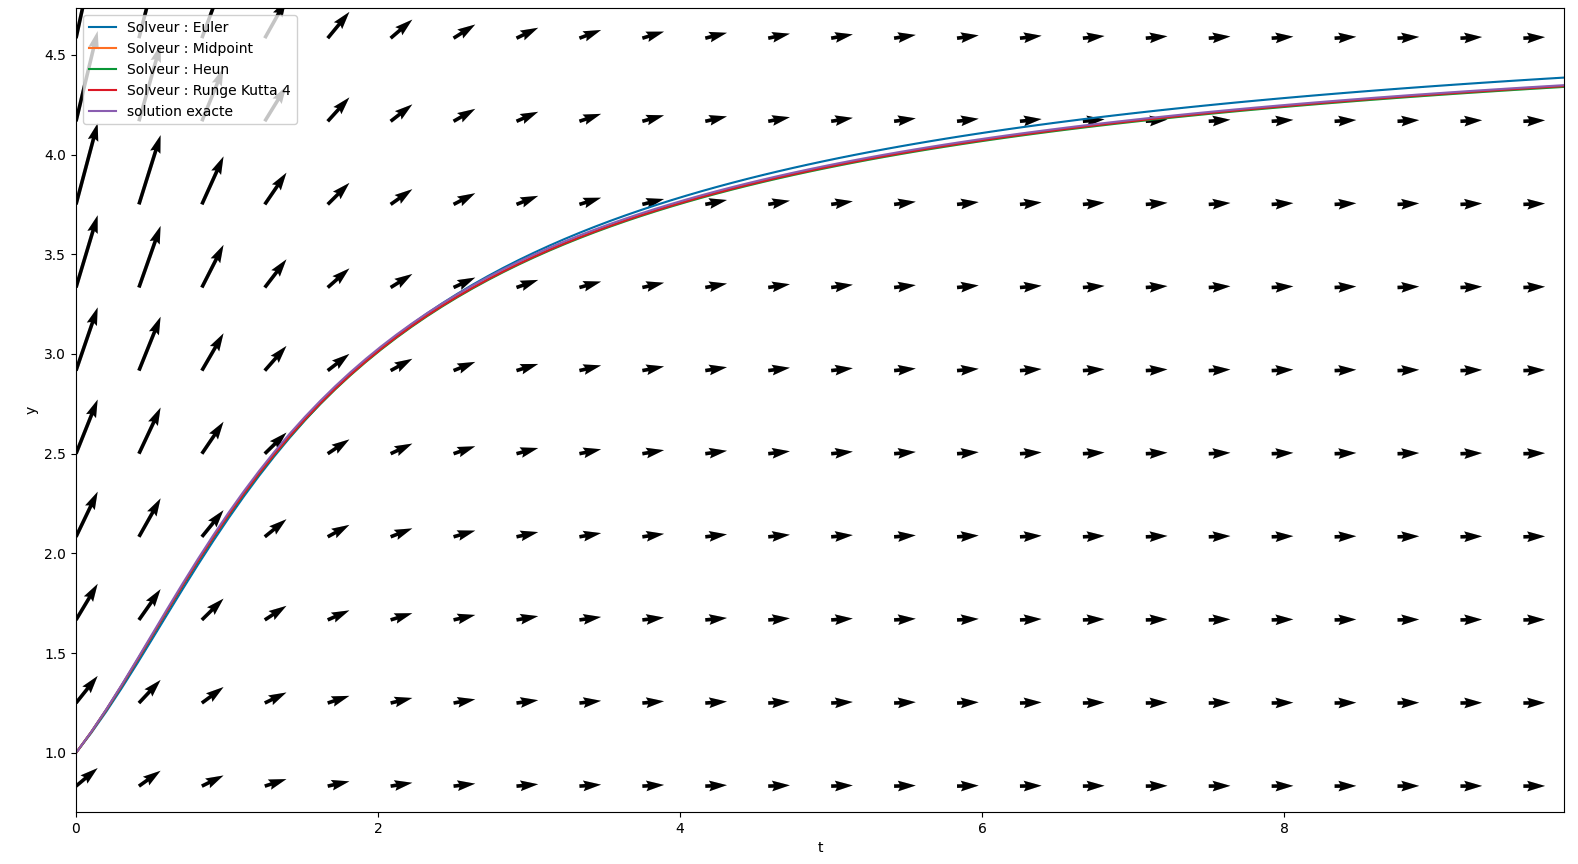
\includegraphics[width=0.49\textwidth]{img/ode1}
		\label{fig:solver_1d}
	}
	\subfloat[Résolution de $\begin{cases}
		y_1' = -y_2\\
		y_2' = y1\\
		y_1(0) = 1 \text{et} y_2(0) = 0
	\end{cases}$]{
		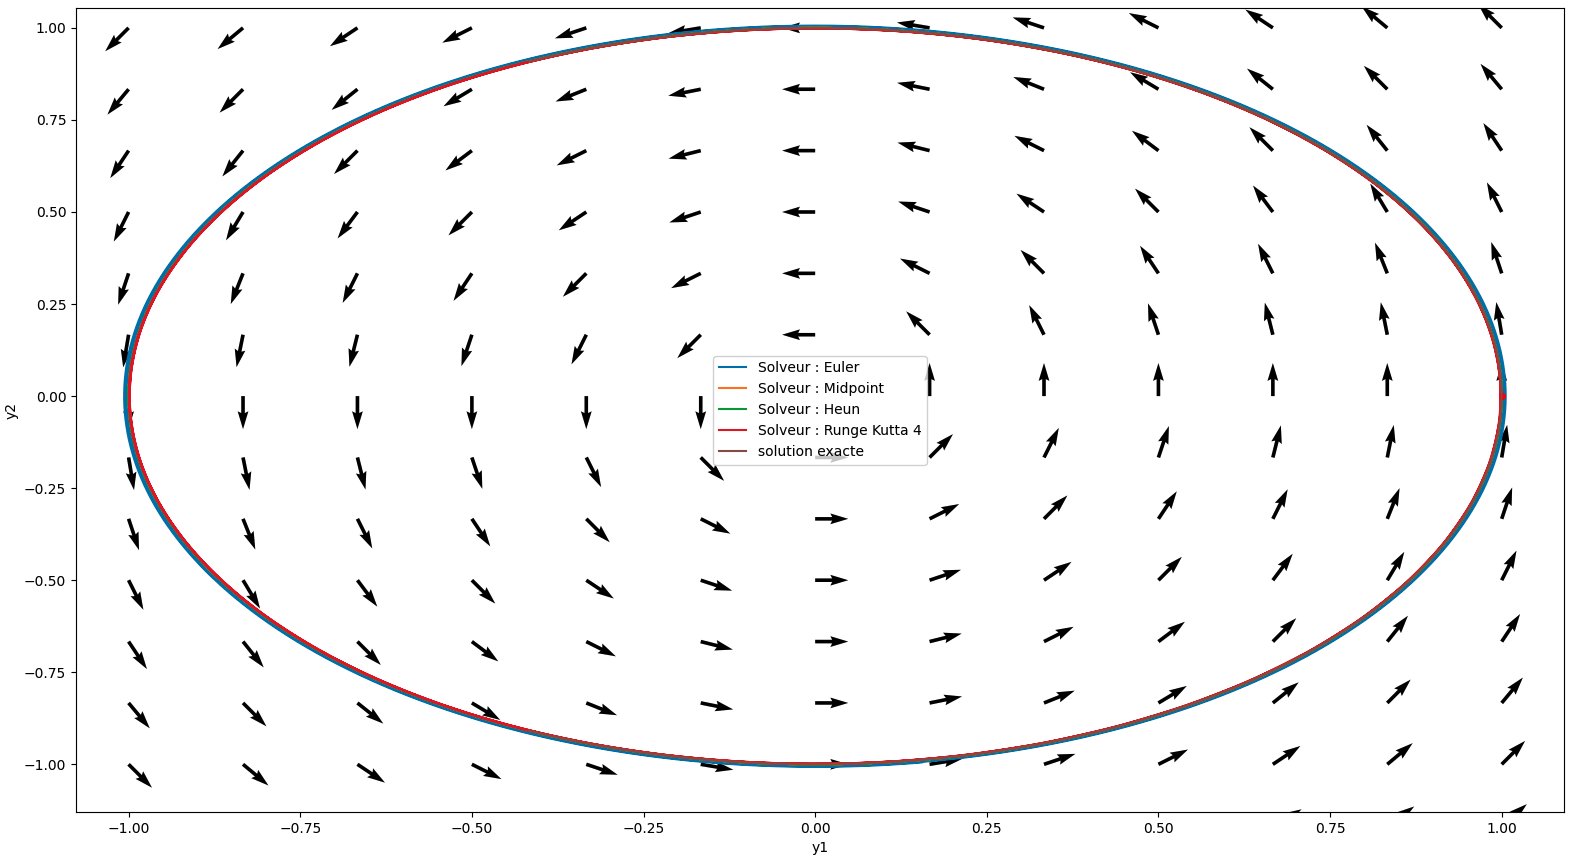
\includegraphics[width=0.49\textwidth]{img/ode2}
		\label{fig:solver_2d}
	}
	\caption{Exemples de résolution de systèmes d'équations différentielles}
	\label{fig:solver_test}
\end{figure}

On remarque en particulier que, sur la figure~\ref{fig:solver_1d}, la méthode d'Euler est bien moins performante que les autres méthodes. Cela s'explique notamment car la méthode est d'ordre 1. La méthode de Runge-Kutta étant d'ordre 4, celle-ci doit alors être préférée aux autres.